\section{Module 11. Brain 3D}

\indent To prepare tree dimension visualization of the cerebral cortex algorithm of marching cubes
is used.\\
 \indent The input data is multiple 2D slices of MR image. The marching cubes algorithm create a polygonal representation of constant density surfaces from a 3D array of data. To select the cerebral cortex is used output data from segmentation made in module 9. The structure of cortex is represented by value 3 in segmentation mask. 
\indent The space of the image is divided into a regular grid of cubes. In each iteration one cube is considered. At each vertex of cube is determined how the surface intersects this cube. The density value are compared with the limit value - surface constant. If the data value is bigger than suface constant, one is assinged to a cube’s vertex. There are 256 combinations of cube orientation relative to the surface, but we can distinguish 15 basic patterns, that repeat as symmetrical reflections, produces all possibilities (Fig. \ref{fig:figures/Marching cubes}). If all values are less than the constant value, then the cube does not form any polygon. Otherwise, the edges of the polygon are defined (by linear interpolation) at the edges that intersect the surface. Using central differences, a unit normal at each cube vertex is calculated and then normal to each trangle vertex is interpolated. The output of the algorithm is the triangle vertices and vertex normals.

\begin{figure}[H]
\centering{}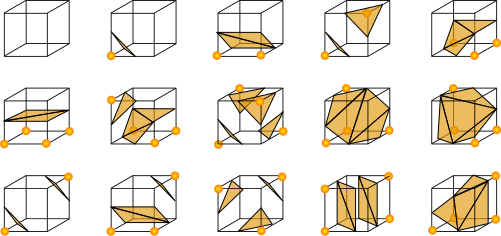
\includegraphics[scale=0.7]{figures/MarchingCubes}\caption{Triangulation for the 15 patterns. \label{fig:figures/Marching cubes}}
\end{figure}

\indent To visualization the model, obtained by marching cubes, the
VTK library is used, which enables building the three-dimension model.
The VTK is object-oriented library. The classes of VTK is dedicated to processing and visualization data.
\\
 \indent The second part of this module includes visualization of the brain’s cross-section on arbitrarily defined plane. To enable selecting of intersection plane there was used object of VTK class, which allows set plane in elected direction by using computer mouse. When the plane is moved by user, in the real time the  three-dimensional model is clipped in the place of selected plane. To improve quality of visualization the cross-section image, there is also possibility to see the image imposed on the three-dimensional model. \\

